%%% License: Creative Commons Attribution Share Alike 4.0 (see https://creativecommons.org/licenses/by-sa/4.0/)


%%%%%%%%%%%%%%%%%%%%%%%%%%%%%%%%%%%%%%%%%

%----------------------------------------------------------------------------------------
%	PACKAGES AND OTHER DOCUMENT CONFIGURATIONS
%----------------------------------------------------------------------------------------

\documentclass{article}

\usepackage{amssymb}
\usepackage{enumerate}
\usepackage[usenames,dvipsnames]{color}
\usepackage{fancyhdr} % Required for custom headers
\usepackage{lastpage} % Required to determine the last page for the footer
\usepackage{extramarks} % Required for headers and footers
\usepackage[usenames,dvipsnames]{color} % Required for custom colors
\usepackage{graphicx} % Required to insert images
\usepackage{listings} % Required for insertion of code
\usepackage{courier} % Required for the courier font
\usepackage[table]{xcolor}
\usepackage{amsfonts,amsmath,amsthm,parskip,setspace,url}
\usepackage[section]{placeins}
\usepackage[a4paper]{geometry}
\usepackage[USenglish]{babel}
\usepackage[utf8]{inputenc}


% Margins
\topmargin=-0.45in
\evensidemargin=0in
\oddsidemargin=0in
\textwidth=6.5in
\textheight=9.0in
\headsep=0.6in

\linespread{1.1} % Line spacing

%----------------------------------------------------------------------------------------
%	DOCUMENT STRUCTURE COMMANDS
%	Skip this unless you know what you're doing
%----------------------------------------------------------------------------------------

% Header and footer for when a page split occurs within a problem environment
\newcommand{\enterProblemHeader}[1]{
\nobreak\extramarks{#1}{#1 continued on next page\ldots}\nobreak
\nobreak\extramarks{#1 (continued)}{#1 continued on next page\ldots}\nobreak
}

% Header and footer for when a page split occurs between problem environments
\newcommand{\exitProblemHeader}[1]{
\nobreak\extramarks{#1 (continued)}{#1 continued on next page\ldots}\nobreak
\nobreak\extramarks{#1}{}\nobreak
}

\setcounter{secnumdepth}{0} % Removes default section numbers
\newcounter{homeworkProblemCounter} % Creates a counter to keep track of the number of problems

\newcommand{\homeworkProblemName}{}
\newenvironment{ex}[1][Problem \arabic{homeworkProblemCounter}]{ % Makes a new environment called homeworkProblem which takes 1 argument (custom name) but the default is "Problem #"
\stepcounter{homeworkProblemCounter} % Increase counter for number of problems
\renewcommand{\homeworkProblemName}{#1} % Assign \homeworkProblemName the name of the problem
\section{\homeworkProblemName} % Make a section in the document with the custom problem count
%\enterProblemHeader{\homeworkProblemName} % Header and footer within the environment
}{
%\exitProblemHeader{\homeworkProblemName} % Header and footer after the environment
}

\newcommand{\problemAnswer}[1]{ % Defines the problem answer command with the content as the only argument
\noindent\framebox[\columnwidth][c]{\begin{minipage}{0.98\columnwidth}#1\end{minipage}} % Makes the box around the problem answer and puts the content inside
}

\newcommand{\homeworkSectionName}{}
\newenvironment{homeworkSection}[1]{ % New environment for sections within homework problems, takes 1 argument - the name of the section
\renewcommand{\homeworkSectionName}{#1} % Assign \homeworkSectionName to the name of the section from the environment argument
\subsection{\homeworkSectionName} % Make a subsection with the custom name of the subsection
%\enterProblemHeader{\homeworkProblemName\ [\homeworkSectionName]} % Header and footer within the environment
}{
%\enterProblemHeader{\homeworkProblemName} % Header and footer after the environment
}

\newif\ifsolutions

%----------------------------------------------------------------------------------------
%----------------------------------------------------------------------------------------
%----------------------------------------------------------------------------------------
% Set up the header and footer
\pagestyle{fancy}
\lhead[c]{\textbf{{\color[rgb]{.5,0,0} K{\o}benhavns\\Universitet }} \firstxmark} % Top left header
\chead{\textbf{{\color[rgb]{.5,0,0} \Class }}\\ \hmwkTitle  } % Top center head
\rhead{\instructor \\ \theprofessor} % Top right header
\lfoot{\lastxmark} % Bottom left footer
\cfoot{} % Bottom center footer
\rfoot{Page\ \thepage\ of\ \protect\pageref{LastPage}} % Bottom right footer
\renewcommand\headrulewidth{0.4pt} % Size of the header rule
\renewcommand\footrulewidth{0.4pt} % Size of the footer rule

\setlength\parindent{0pt} % Removes all indentation from paragraphs







%----------------------------------------------------------------------------------------
%	NAME AND CLASS SECTION
%----------------------------------------------------------------------------------------

\newcommand{\hmwkTitle}{Exercises: Lec 2b} % Assignment title
\newcommand{\Class}{Mechanism Design} % Course/class
\newcommand{\instructor}{Fall 2019} % TA
\newcommand{\theprofessor}{Prof. Egor Starkov} % Professor

%\theoremstyle{definition} \newtheorem{ex}{\textbf{\Large{Exercise & #}\\}}
\setlength{\parskip}{0 pt}




















%%%%%%%%%%%%%%%%%%%%%%%%%%%%%%%%%%%%%%%%%%%%%%%%%%%%%%%%%%%%%%%%%%%%%%%%%%%%%%%%%%%%%%
\solutionsfalse
%\solutionstrue
%%%%%%%%%%%%%%%%%%%%%%%%%%%%%%%%%%%%%%%%%%%%%%%%%%%%%%%%%%%%%%%%%%%%%%%%%%%%%%%%%%%%%%


\begin{document}
	
These exercises are for your own practice and are not to be handed in. Some exercises are open ended in that they may not have a unique correct answer.

%%------------------------------------------------------------------------------------------------

\begin{ex}[Review Questions]
	\begin{itemize}
		\item The Groves-Clarke mechanism implements the efficient allocation in dominant stratgies. Why does this not violate the Gibbard-Satterthwaite theorem?
		\item Why is it a dominant strategy in the VCG mechanism to reveal one’s true type? What is the idea behind the mechanism? Why are VCG transfers sometimes called "externality transfers"?
		\item What is the fundamental tension between the requirements of Individual Rationality and Budget Balance?
		\item In which sense is monotonicity requirement (for an s.c.f. to be DSIC in a Euclidean model) related to WPRP condition from the general model?
		\item What is the main driving force behind revenue equivalence? Does it imply that the expected revenue and players' expected payoffs are fixed given a social choice function?
	\end{itemize}
	
\end{ex}



%%------------------------------------------------------------------------------------------------

\begin{ex}[Implementability conditions]
	In the Euclidean world we showed that monotonicity and the Mirrlees conditions were necessary for an indirect utility function to arise from a DSIC mechanism. Show sufficiency:  for any indirect utility function $U$ that satisfies monotonicity and the Mirrlees condition there is a DSIC social choice function which yields $U$.
	
	\ifsolutions
	\section*{Solution}
	See the lemma in ``implementability in auctions'' problem.
	\fi
\end{ex}



%%------------------------------------------------------------------------------------------------

\begin{ex}[Budget balance]
	Prove that if a mechanism is ex post budget balanced then it is also ex ante budget balanced.
	
	\ifsolutions
	\section*{Solution}
	If any
	\fi
\end{ex}



%%------------------------------------------------------------------------------------------------

\begin{ex}[Bilateral trade]
	Is there an efficient, DSIC, ex post IR, ex post BB mechanism in the bilateral trade setting (slides 68/83)? (Hint: Start from VCG and invoke revenue equivalence.)
	
	\ifsolutions
	\section*{Solution}
	If any
	\fi
\end{ex}



%%------------------------------------------------------------------------------------------------

\begin{ex}[Implementation in Auctions]
	Consider the auction environment with two buyers.  Suppose that each buyer $i$ has willingness to pay
	$v_i$ drawn from the set $[0,1].$
	\begin{enumerate}
		\item Draw a square with $v_1$ on the horizontal axis and $v_2$ on the vertical axis.  A point in the square
		represents a profile $(v_1, v_2)$.
		\item Draw a downward sloping curve through the box.
		\item Draw an upward sloping curve through the box that intersects the downward sloping curve (exactly once.)
		\item The region above your downward sloping curve is divided into two subregions by your upward sloping curve.  Label
		the subregion that is above your upward sloping curve with a $2$ and label the other subregion with a $1$.  Label
		the entire region that is below (and to the left of) your downward sloping curve with a $0$.
		\item Consider the allocation rule that is defined by your drawing.  In the $1$ region agent $1$ gets the
		good, in the $2$ region agent $2$ gets the good and in the $0$ region neither agent gets the good.  (On the boundary
		between regions pick the allocation from one of the neighboring regions. )  Find a transfer rule which, when
		coupled with your allocation rule, forms a DSIC mechanism.
		\item Is there any DSIC allocation rule that picks alternatives from the set $\{0,1,2\}$ that could not be represented
		by a drawing that follows the instructions given above?
	\end{enumerate}
	
	\ifsolutions
	\section*{Solution}
	Before solving the exercise we will show the following claim. Consider the environment as the one in the instructions, where the utility of type $v_i$ when he announces $v_i^{'}$ and his rival announces $v_{-i}$ is:
	\begin{eqnarray}
	U_{i}(v_i^{'}|v_{i})=v_iq_i(v_{i}^{'},v_{-i})-t_i(v_{i}^{'},v_{-i})\\
	U_i(v_{i})=U_i(v_i|v_i)
	\end{eqnarray}
	where $q_i(v_{i}^{'},v_{-i})\in[0,1]$ is the probability that $i$ gets the good when the announcements are $(v_i^{'},v_{-i})$ and $t_i(v_{i}^{'},v_{-i})$ are the payments that need to be done by $i$ in that case.
	\begin{lem}
		A mechanism $(q(\cdot),t(\cdot))$ is DSIC if for all $i,v_{-i}$ $q_{i}(\cdot,v_{-i})$ is weakly increasing. Moreover,
		\begin{eqnarray}\label{int}
		U_{i}(v_i)=U_i(\underbar{v}_{i})+\int_{\underbar{v}_{i}}^{v_i}q_{i}(u,v_{-i})du
		\end{eqnarray}
		Moreover, if $q(\cdot)$ is such that for all $i,v_{-i}$ $q_{i}(\cdot,v_{-i})$ is weakly increasing and satisfies (\ref{int}), then it is DSIC.
	\end{lem}
	\begin{proof}
		\begin{description}
			\item [($\Rightarrow$)] Suppose $(q(\cdot),t(\cdot))$ is DSIC. Then, for all $i,v_i$ it holds that:
			\begin{eqnarray}
			U_i(v_i)\geq U_i(v_i^{'}|v_i)\\
			U_i(v_{i}^{'})\geq U_i(v_i|v_i^{'})
			\end{eqnarray}
			Note that: $U_i(v_i^{'}|v_i)=U_i(v_{i}^{'}|v_{i}^{'})+(v_i-v_i^{'})q_i(v_i^{'},v_{-i})$ and $U_i(v_i|v_i^{'})=U_i(v_{i}|v_{i})+(v_i^{'}-v_i)q_i(v_i,v_{-i})$. Then we may rewrite the above inequalities as:
			\begin{eqnarray}
			U_i(v_i)\geq U_i(v_i^{'}|v_i)=U_i(v_{i}^{'}|v_{i}^{'})+(v_i-v_i^{'})q_i(v_i^{'},v_{-i})\\
			U_i(v_{i}^{'})\geq U_i(v_i|v_i^{'})=U_i(v_{i}|v_{i})+(v_i^{'}-v_i)q_i(v_i,v_{-i})
			\end{eqnarray}
			Rearranging, we obtain that:
			\begin{eqnarray}
			(v_i-v_{i}^{'})q_i(v_i^{'},v_{-i})\leq U_i(v_i)-U_{i}(v_i^{'})\leq (v_i-v_{i}^{'})q_i(v_i,v_{-i})
			\end{eqnarray}
			Assume, wlog, that $v_i>v_i^{'}$. Then, the above inequality implies that $q_i(v_i,v_{-i})\geq q_i(v_i^{'},v_{-i})$ as desired. Moreover, rearranging the inequality we get that:
			\begin{eqnarray}
			q_i(v_i^{'},v_{-i})\leq \frac{U_i(v_i)-U_{i}(v_i^{'})}{(v_i-v_{i}^{'})}\leq q_i(v_i,v_{-i})
			\end{eqnarray}
			and taking limits as $v_{i}^{'}\rightarrow v_i$ we get that:
			\begin{eqnarray}
			U_i^{'}(v_i)= q_i(v_i,v_{-i})
			\end{eqnarray}
			And hence, we may write $U_i(v_i)$ as:
			\begin{eqnarray}
			U_{i}(v_i)=U_i(\underbar{v}_{i})+\int_{\underbar{v}_{i}}^{v_i}q_{i}(u,v_{-i})du
			\end{eqnarray}
			for $\underbar{v}_i<v_i$.
			\item [($\Leftarrow$)] Assume you have an allocation $q(\cdot)$ that is weakly increasing and satisfies (\ref{int}). Then, construct transfers as:
			\begin{eqnarray}
			t_i(v_i,v_{-i})=v_iq_i(v_i,v_{-i})-U_i(\underbar{v}_{i})-\int_{\underbar{v}_{i}}^{v_i}q_{i}(u,v_{-i})du
			\end{eqnarray}
			We will show that $(q,t)$ is DSIC. Fix $v_{-i}$ and let $v_i>v_{i}^{'}$. Then:
			\begin{eqnarray}
			U_i(v_i)-U_{i}(v_i^{'})= \int_{v^{'}_{i}}^{v_i}q_{i}(u,v_{-i})du\geq \int_{v^{'}_{i}}^{v_i}q_{i}(v_{i}^{'},v_{-i})du=(v_i-v_i^{'})q_i(v_i^{'},v_{-i})
			\end{eqnarray}
			where we used the monotonicity of $q_i$ to get the inequality. Hence,
			\begin{eqnarray}
			U_i(v_i)\geq v_iq_i(v_i^{'},v_{-i})-(v_i^{'}q_i(v_i^{'},v_{-i})-U_i(v_i^{'}))=v_iq_i(v_i^{'},v_{-i})-t_i(v_i^{'},v_{-i})
			\end{eqnarray}
			where we used the constructed transfers to get the last equality. Hence, the mechanism is DSIC.
		\end{description}
	\end{proof}
	From now on, we will work 	with the following figure:
	\begin{center}
		\begin{figure}[htbp]
			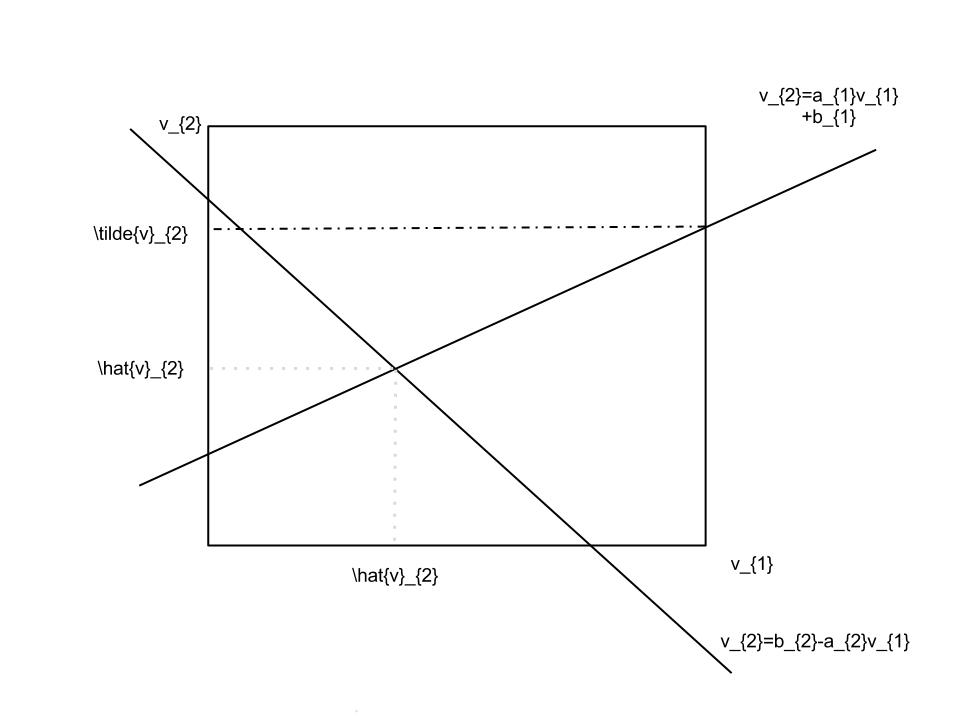
\includegraphics[scale=0.5]{./ps2}
		\end{figure}
	\end{center}
	\newpage
	\paragraph\indent Of course, there will be some things that are specific to the drawing, but the way we will solve the exercise (mainly, by using the result above) should illustrate the general procedure for different figures. Based on the figure, we construct the following allocation:
	\[q_1(v_1,v_2)=\left\{\begin{array}{cc} 0 & \text{ if } v_2+a_2v_1\leq b_2\quad \text{ or }\quad v_2\geq b_1+a_1v_1\\
	1 & \quad\text{otherwise}\quad
	
	\end{array}
	\right.
	\]
	\[q_2(v_1,v_2)=\left\{\begin{array}{cc} 0 & \text{ if } v_2+a_2v_1\leq b_2\quad \text{ or }\quad v_2\leq b_1+a_1v_1\\
	1 & \quad\text{otherwise}\quad
	
	\end{array}
	\right.
	\]
	\newline\indent From the lemma above we know that we have no hope of implementing the allocation if it is not monotone. However, it is very easy to check (just observe the drawing) that fixing the type of the other player, the probability of getting the good weakly increases with the player's type. Now we have to construct the transfers to implement this in dominant strategies. We will make use once again of the lemma, mainly of the result that:
	\begin{eqnarray}\label{transfer}
	t_i(v_i,v_{-i})=v_iq_i(v_i,v_{-i})-U_i(\underbar{v}_{i})+\int_{\underbar{v}_{i}}^{v_i}q_{i}(u,v_{-i})du
	\end{eqnarray}
	are the transfers that work.
	\newline\indent Let's start with $t_1(v_1,v_2)$. Note that if $v_2>\tilde{v}_2$, no matter what type player 1 announces $q_1(\cdot,v_2)=0$. Hence, $t_1(v_1,v_2)=0$ for $v_2>\tilde{v}_2$. Consider now $v_2\in[\hat{v}_2,\tilde{v}_2]$. In that case, $q_1(v_1,v_2)=1$ if and only if $v_1\geq\frac{v_2-b_1}{a_1}$. Then,  for $v_2\in[\hat{v}_2,\tilde{v}_2]$:
	
	\[t_1(v_1,v_2)=\left\{\begin{array}{cc} 0 & \quad\text{ if }\quad  v_1\leq\frac{v_2-b_1}{a_1}\\
	\frac{v_2-b_1}{a_1} & \quad\text{otherwise}\quad
	
	\end{array}
	\right.
	\]
	where the last part comes from using (\ref{transfer}) and noticing that $\underbar{v}_1=\frac{v_2-b_1}{a_1}$ and setting $U_1(\underbar{v}_1)=0$:
	\begin{eqnarray}
	t_1(v_1,v_2)=v_1-\int_{\frac{v_2-b_1}{a_1}}^{v_1}1 du=\frac{v_2-b_1}{a_1}
	\end{eqnarray}
	Finally, consider $v_2\leq\hat{v}_2$. In that case, $q_1(\cdot,v_2)=0$ for $v_1\leq \frac{b_2-v_2}{a_2}=\underbar{v}_1$. Then, in that case:
	
	\[t_1(v_1,v_2)=\left\{\begin{array}{cc} 0 & \quad\text{ if }\quad  v_1\leq\frac{b_2-v_2}{a_2}\\
	\frac{b_2-v_2}{a_2} & \quad\text{otherwise}\quad
	
	\end{array}
	\right.
	\]
	\newline\indent Notice that, apart from the result of the lemma saying it is the case, it is clear why the mechanism is DSIC: whether the player pays or not depends on his announcement, but not how much he pays. In this much, it is like a SPA.
	\newline\indent We can calculate the transfers for player 2 in a similar manner. Consider $v_1<\hat{v}_1$. Then, $q_2(v_1,v_2)=0$ if $v_2\leq b_2-a_2 v_1$. Then,
	
	\[t_2(v_1,v_2)=\left\{\begin{array}{cc} 0 & \quad\text{ if }\quad  v_2\leq b_2-a_2 v_1\\
	b_2-a_2 v_1 & \quad\text{otherwise}\quad
	
	\end{array}
	\right.
	\]
	On the other hand, if $v_1\geq\hat{v}_1$, we have that $q_2(v_1,v_2)=0$ if $v_2\leq a_1v_1+b_1$. Then:
	\[t_2(v_1,v_2)=\left\{\begin{array}{cc} 0 & \quad\text{ if }\quad  v_2\leq b_1+a_1 v_1\\
	b_1+a_1 v_1 & \quad\text{otherwise}\quad
	
	\end{array}
	\right.
	\]
	\fi
\end{ex}



%%------------------------------------------------------------------------------------------------

%TODO: this is for correlated types
%\begin{ex}[Asymmetric Auctions]
%	Consider the optimal auction problem in which there are two bidders whose valuations $v_i \in [0,1]$ are uniformly distributed but perfectly correlated, i.e. $v_1 = v_2$ with probability 1.  Construct a DSIC mechanism with the following properties:
%	\begin{enumerate}
%		\item Bidder 2 wins the object regardless of the type profile.
%		\item Both bidders earn zero utility at every type profile.
%	\end{enumerate}
%	
%	\ifsolutions
%	\section*{Solution}
%	Consider the following allocation:
%	\[q_1(v_1,v_2)=0\]
%	\[q_2(v_1,v_2)=\left\{\begin{array}{cc} 0 & \text{ if }\quad v_2\neq v_1\\
%	1 & \quad\text{otherwise}\quad
%	
%	\end{array}
%	\right.\]
%	\[t_1(v_1,v_2)=0\]
%	\[t_2(v_1,v_2)=\left\{\begin{array}{cc} 0 & \text{if}\quad v_2\neq v_1\\
%	v_1 & \quad\text{otherwise}\quad\end{array}\right.\]
%	Note that for bidder 1 it is weakly dominant to say his valuation: he never gets the good so he might as well say $v_1$. For player 2, we have exactly the same situation: given the message sent by agent 1, he is indifferent between saying the truth and not, so telling the truth is weakly dominant. Agent 2 gets the good always and both bidders have 0 utility at every profile.
%	\fi
%\end{ex}



%%------------------------------------------------------------------------------------------------

\end{document}
